%%%%%%%%%%%%%%%%%%%%%%%%%%%%%%%%%%%%%%%%%
% Beamer Presentation
% LaTeX Template
% Version 1.0 (10/11/12)
%
% This template has been downloaded from:
% http://www.LaTeXTemplates.com
%
% License:
% CC BY-NC-SA 3.0 (http://creativecommons.org/licenses/by-nc-sa/3.0/)
%
%%%%%%%%%%%%%%%%%%%%%%%%%%%%%%%%%%%%%%%%%

%----------------------------------------------------------------------------------------
%	PACKAGES AND THEMES
%----------------------------------------------------------------------------------------

\documentclass{beamer}

\mode<presentation> {

% The Beamer class comes with a number of default slide themes
% which change the colors and layouts of slides. Below this is a list
% of all the themes, uncomment each in turn to see what they look like.

%\usetheme{default}
%\usetheme{AnnArbor}
%\usetheme{Antibes}
%\usetheme{Bergen}
%\usetheme{Berkeley}
%\usetheme{Berlin}
%\usetheme{Boadilla}
%\usetheme{CambridgeUS}
%\usetheme{Copenhagen}
%\usetheme{Darmstadt}
%\usetheme{Dresden}
%\usetheme{Frankfurt}
%\usetheme{Goettingen}
%\usetheme{Hannover}
%\usetheme{Ilmenau}
%\usetheme{JuanLesPins}
%\usetheme{Luebeck}
\usetheme{Madrid}
%\usetheme{Malmoe}
%\usetheme{Marburg}
%\usetheme{Montpellier}
%\usetheme{PaloAlto}
%\usetheme{Pittsburgh}
%\usetheme{Rochester}
%\usetheme{Singapore}
%\usetheme{Szeged}
%\usetheme{Warsaw}

% As well as themes, the Beamer class has a number of color themes
% for any slide theme. Uncomment each of these in turn to see how it
% changes the colors of your current slide theme.

%\usecolortheme{albatross}
%\usecolortheme{beaver}
%\usecolortheme{beetle}
%\usecolortheme{crane}
%\usecolortheme{dolphin}
%\usecolortheme{dove}
%\usecolortheme{fly}
%\usecolortheme{lily}
%\usecolortheme{orchid}
%\usecolortheme{rose}
%\usecolortheme{seagull}
%\usecolortheme{seahorse}
%\usecolortheme{whale}
%\usecolortheme{wolverine}

%\setbeamertemplate{footline} % To remove the footer line in all slides uncomment this line
%\setbeamertemplate{footline}[page number] % To replace the footer line in all slides with a simple slide count uncomment this line

%\setbeamertemplate{navigation symbols}{} % To remove the navigation symbols from the bottom of all slides uncomment this line
}

\usepackage{graphicx} % Allows including images
\usepackage{booktabs} % Allows the use of \toprule, \midrule and \bottomrule in tables
\usepackage{cite}     % Citation package
\usepackage{amsmath,amssymb,amsfonts} %AMS Math package
\usepackage{algorithmic}
\usepackage{sistyle}    %SI unit style
\usepackage{romannum}   %Roman numbering style
\usepackage{gensymb}    %math symbol
\usepackage{url}        %URL

%----------------------------------------------------------------------------------------
%	TITLE PAGE
%----------------------------------------------------------------------------------------

\title[SALSA]{SALSA is an ICT based educational tool for Astrophysics students to study structure and dynamics of Milky Way Galaxy } % The short title appears at the bottom of every slide, the full title is only on the title page

\author{Mir Sakhawat Hossain} % Your name
\institute[KNGC] % Your institution as it will appear on the bottom of every slide, may be shorthand to save space
{
Kabi Nazrul Govt. College,Dhaka \\ % Your institution for the title page
\medskip
\textit{s.hossain18@gmail.com} \\ % Your email address
\textit{\url{https://gitlab.com/sakhawat18/iccit-2018}} %Gitlab Link
}
\date{\today} % Date, can be changed to a custom date

\begin{document}

\begin{frame}
\titlepage % Print the title page as the first slide
\end{frame}

\begin{frame}
\frametitle{Overview} % Table of contents slide, comment this block out to remove it
\tableofcontents % Throughout your presentation, if you choose to use \section{} and \subsection{} commands, these will automatically be printed on this slide as an overview of your presentation
\end{frame}

%----------------------------------------------------------------------------------------
%	PRESENTATION SLIDES
%----------------------------------------------------------------------------------------

%------------------------------------------------
\section{Primary Discussion} % Sections can be created in order to organize your presentation into discrete blocks, all sections and subsections are automatically printed in the table of contents as an overview of the talk
%------------------------------------------------

\subsection{SALSA} % A subsection can be created just before a set of slides with a common theme to further break down your presentation into chunks

\begin{frame}
\frametitle{Introduction}
ICT based astronomy and astrophysics tools have been developed for decades for undergraduate level use including radio telescopes controllable over the Internet at minimal cost. These radio telescopes can effectively be used to study galactic structure and dynamics. This paper presents an observation to study galaxy dynamics and map its spiral structure which was carried out between galactic coordinate longitudes $6\degree$ to $225\degree$ and latitudes $0\degree$ to $35\degree$ with two low cost $2.3$ meters Haystack model type radio frequency receiving systems called SALSA radio telescopes at Onsala Space Observatory in Sweden which is maintained by Chalmers University of Technology.
\end{frame}
%------------------------------------------------

\begin{frame}
\frametitle{SALSA Telescope}
\begin{figure}
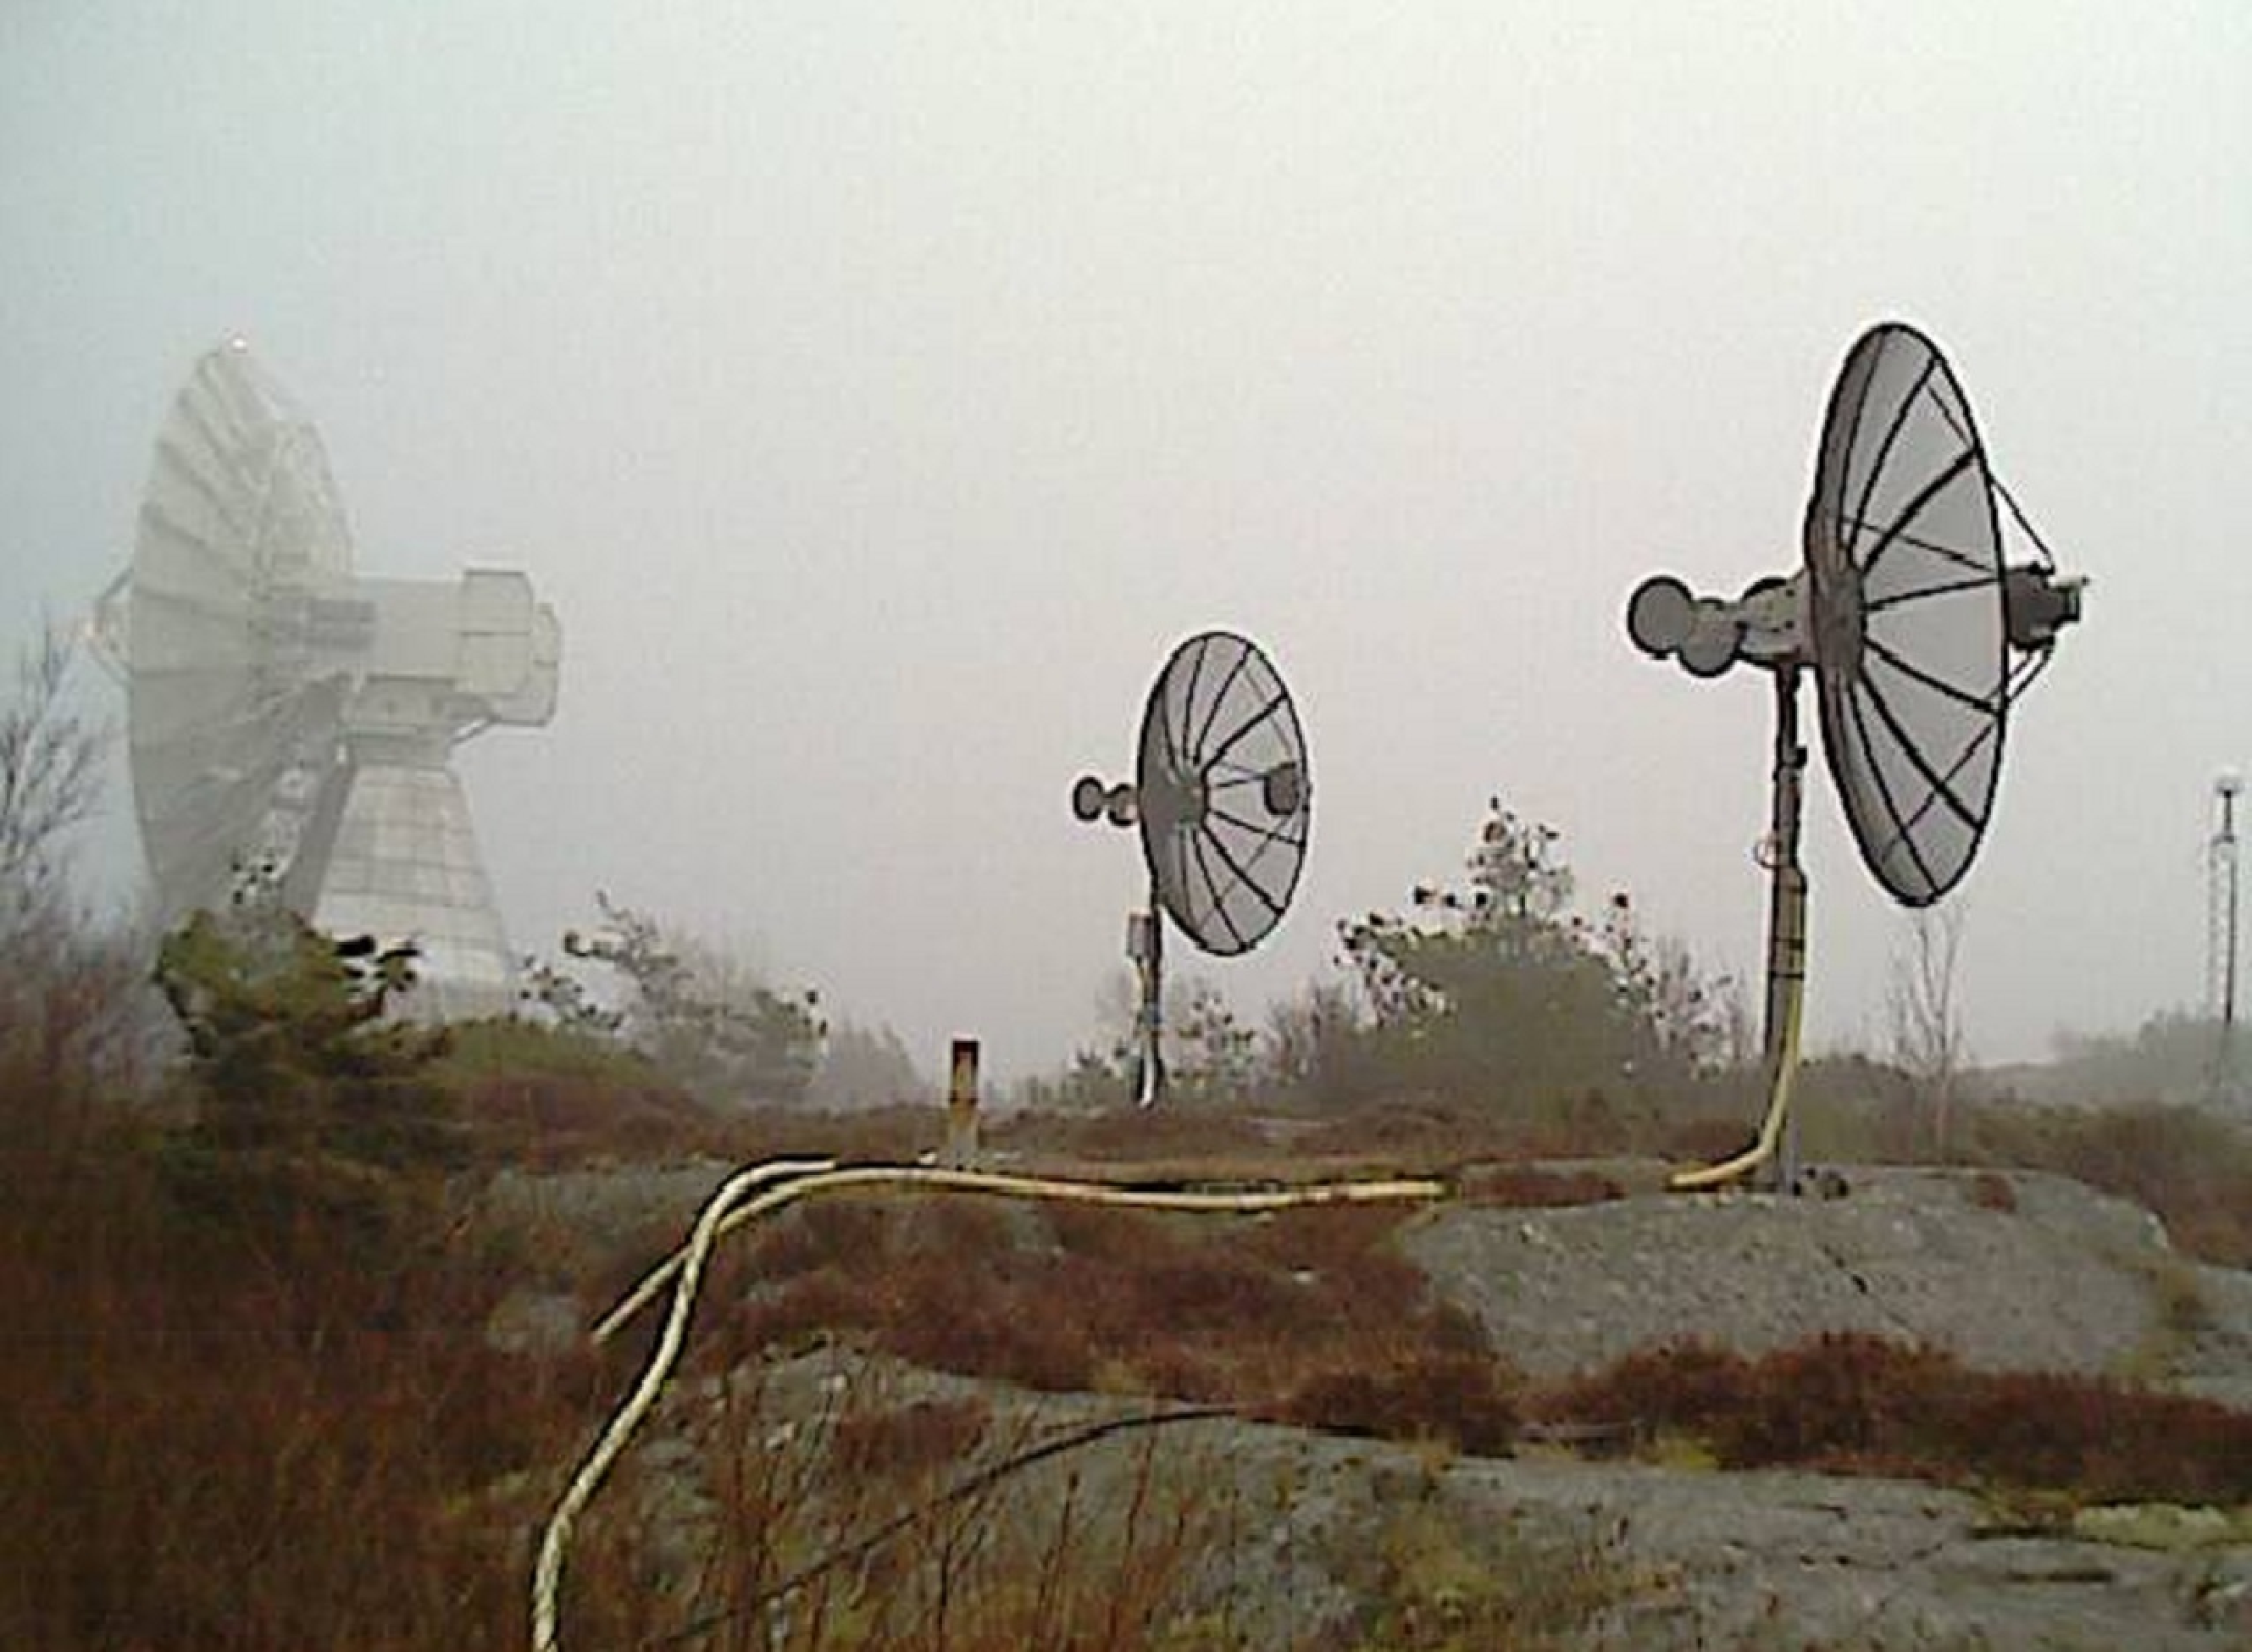
\includegraphics[width=0.7\linewidth]{salsa.png}
\end{figure}
\end{frame}

%------------------------------------------------

\begin{frame}
\frametitle{Basic Details of SALSA}
SALSA is a part of the European Hands-On Universe project(EU-HOU)\cite{Ferlet2006} designed to bring interactive lessons of astronomy to the classroom. There are two SALSA telescopes with the same specification see Table~\ref{Tab:salsa_specification}\cite{ThomasBensby2017}.\\~\\ 
Anyone can control these telescopes using Internet browser by log in \url{https://vale.oso.chalmers.se/salsa/} for free at any time.
\end{frame}
%------------------------------------------------

\begin{frame}
\frametitle{Basic Diagram of a SALSA Small Radio Telescope}
\begin{figure}
\caption{Block Diagram of Haystack Small Radio Telescope\cite{DustinJohnson2012}}
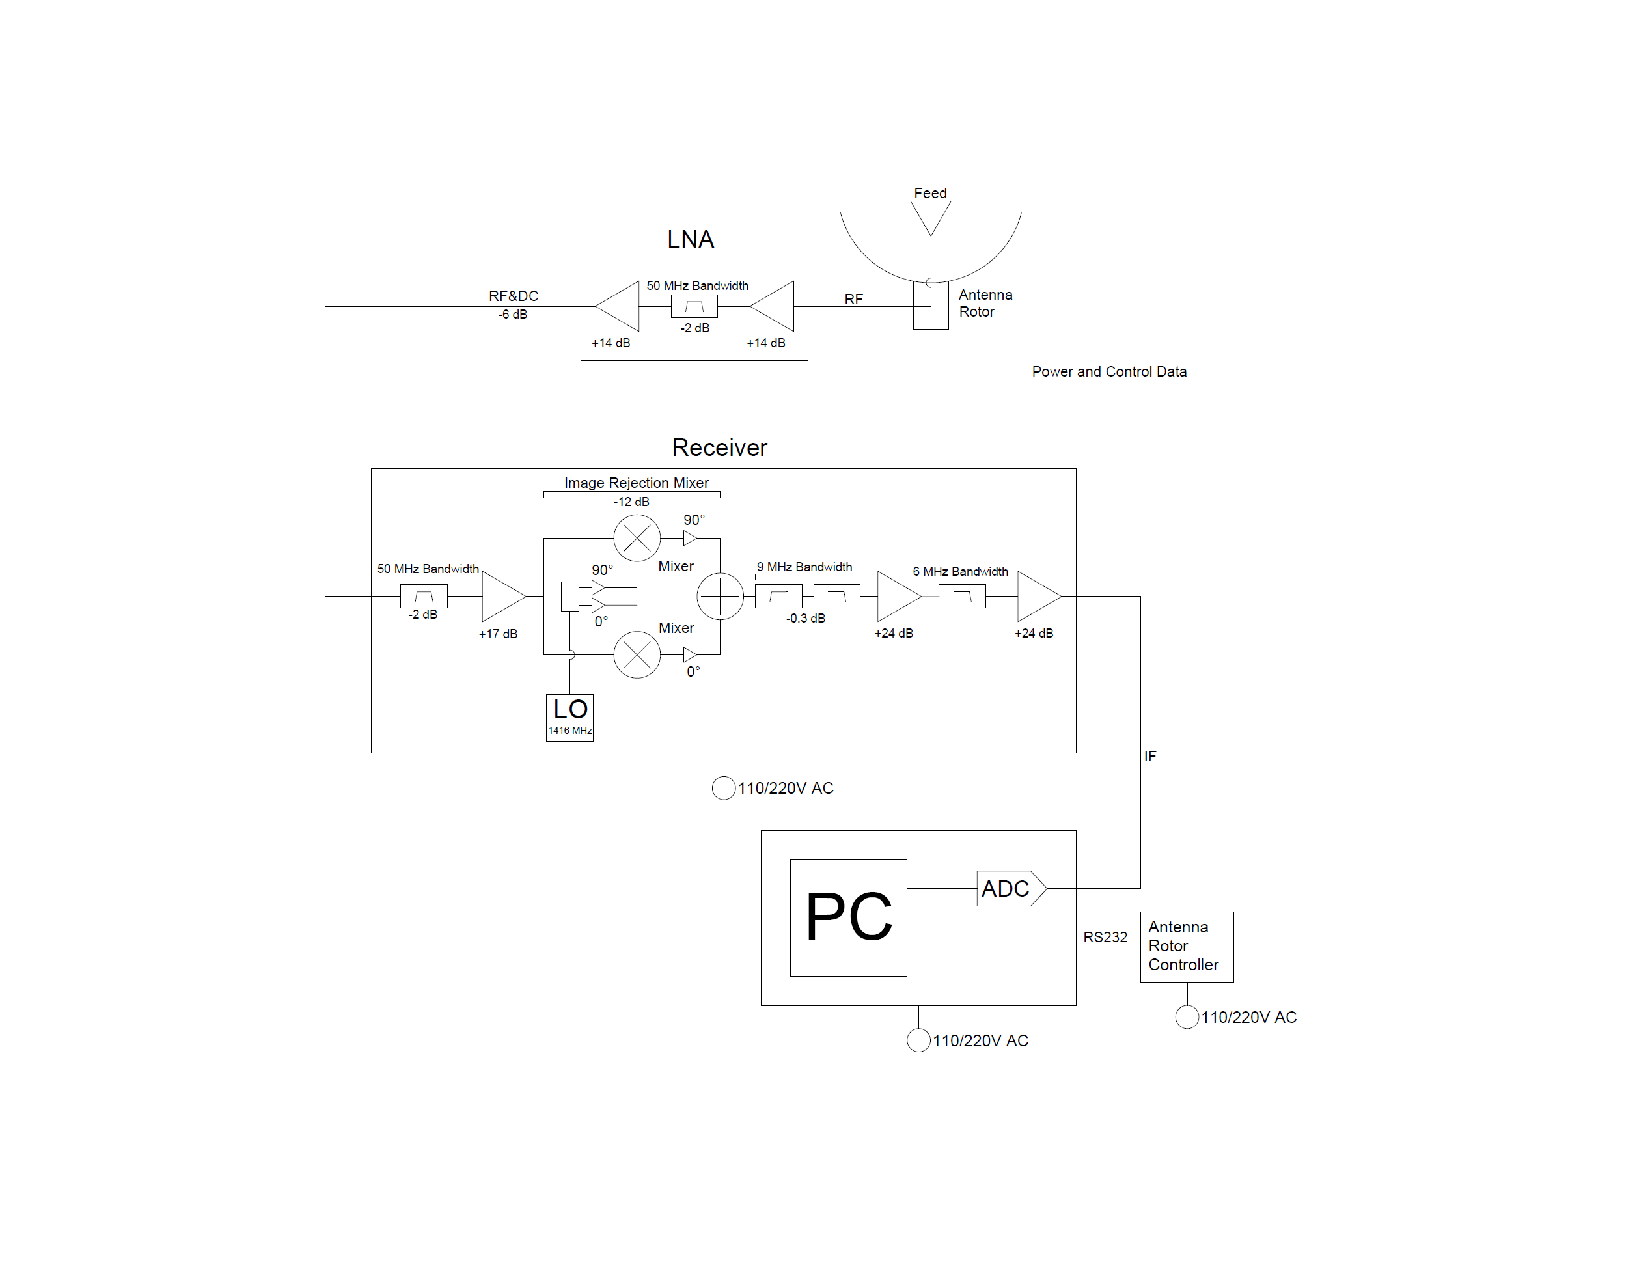
\includegraphics[width=0.8\linewidth]{block}
\end{figure}
\end{frame}

%------------------------------------------------

\begin{frame}
\frametitle{SALSA}
\begin{table}
\caption{Specification of SALSA}
\begin{tabular}{|c|c|}
\hline
\textbf{Parameter}&\multicolumn{1}{|c|}{\textbf{Value}} \\
\cline{1-2} 
\hline
Diameter & 2.3m\\
\hline
Focal Length & 0.9m (f/0.37)\\
\hline
Angular Resolution & 7$\degree$ at 1420MHz\\
\hline
Frequency Range & 1420 $\pm$ 20MHz\\
\hline
Frequency Resolution & 9.375kHz (2.4MHz over 256 Freq. Channels)\\
\hline
Noise Diode Temperature & $\approx$ 100K\\
\hline
System Temperature & $\approx$ 500K\\
\hline
Aperture Efficiency & $\approx$ 50$\%$\\
\hline
Mount & Two-Axis Azimuth/Elevation\\
\hline
Pointing Accuracy & $\approx$ 0.2$\degree$\\
\hline
Travel Limits &  0-90$\degree$ Vertically, 0-360$\degree$ Horizontally\\
\hline
\end{tabular}
\label{Tab:salsa_specification}
\end{table}
\end{frame}
%------------------------------------------------
\begin{frame}
\frametitle{Components of SALSA}
\begin{itemize}
\item A 2.3 meter satellite dish on a fully steerable, motorized azimuth-elevation mount
\item A rotor controller to run the motors which steer the telescope
\item A feed composed of a helical antenna backed by a cavity
\item A super-heterodyne receiver providing 10 MHz bandwidth centered on the 1420.4 MHz (21-cm) hydrogen line
\item A low-noise amplifier
\item A/D conversion on a dedicated PCI card
\item Software on a desktop computer to receive and process data from the telescope and control it
\end{itemize}
\end{frame}

%------------------------------------------------

\subsection{HI Surveys}

%------------------------------------------------
\begin{frame}
\frametitle{HI Surveys}
\begin{columns}[c] % The "c" option specifies centered vertical alignment while the "t" option is used for top vertical alignment

\column{.7\textwidth} % Left column and width
\begin{enumerate}
\item In 1933, Karl Guthe Jansky detected first extraterrestrial radio frequency
\item In 1945 then Van de Hulst predicted $21$ cm wavelength emission
\item Detected HI line by Muller and Oort in the same year
\item A preliminary survey was made by Christiansen and Hindman in Australia
\item In Netherlands, Muller and Westerhout
\item All-sky mapping in HI line based on EBHIS and GASS
\end{enumerate}

\column{.3\textwidth} % Right column and width
Within these periods angular resolution has been developed from $30\degree$ to $30$\,-$\mu$as\cite{kellermann2001development,Middelberg2008}.

\end{columns}
\end{frame}
%------------------------------------------------

%------------------------------------------------

\section{Theory}

%------------------------------------------------

\begin{frame}
\frametitle{Theory}
\begin{theorem}[Hydrogen Line Emission]
\begin{itemize}
\item The frequency of the photon emitted in a transition from the triplet to the singlet state\cite{griffiths2016introduction}\\
$\mathit{\nu}=\frac{\Delta\-E}{h}=\SI{1420}{MHz}$
\item The corresponding wavelength is $c/\nu=21$ cm
\item In a single Hydrogen atom this transition occurs once per $\approx10^{7}$ years 
\item Enormous amount of Hydrogen in spiral arms of Milky Way galaxy causes pervasive and ubiquitous forms of radiation.
\end{itemize}
\end{theorem}
\end{frame}

%------------------------------------------------

\begin{frame}
\frametitle{Hyperfine Splitting of Hydrogen}
\begin{figure}
\caption{21cm Wave Length Hydrogen Line Emission}
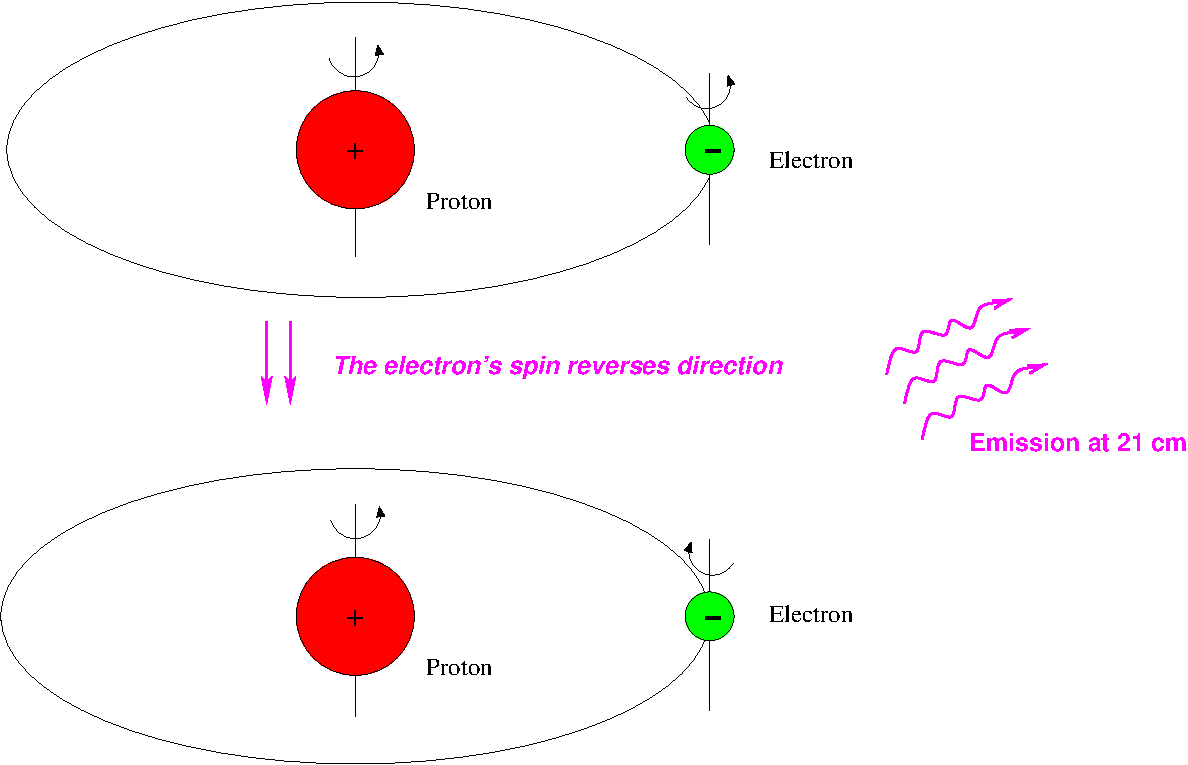
\includegraphics[width=0.8\linewidth]{hyperfine}
\end{figure}
\end{frame}

%------------------------------------------------

\begin{frame}
\frametitle{Spiral Structure of Milky Way Galaxy}
\begin{figure}
\caption{Milky Way(Credit:NASA/JPL-Caltech/ESO/R. Hurt)}
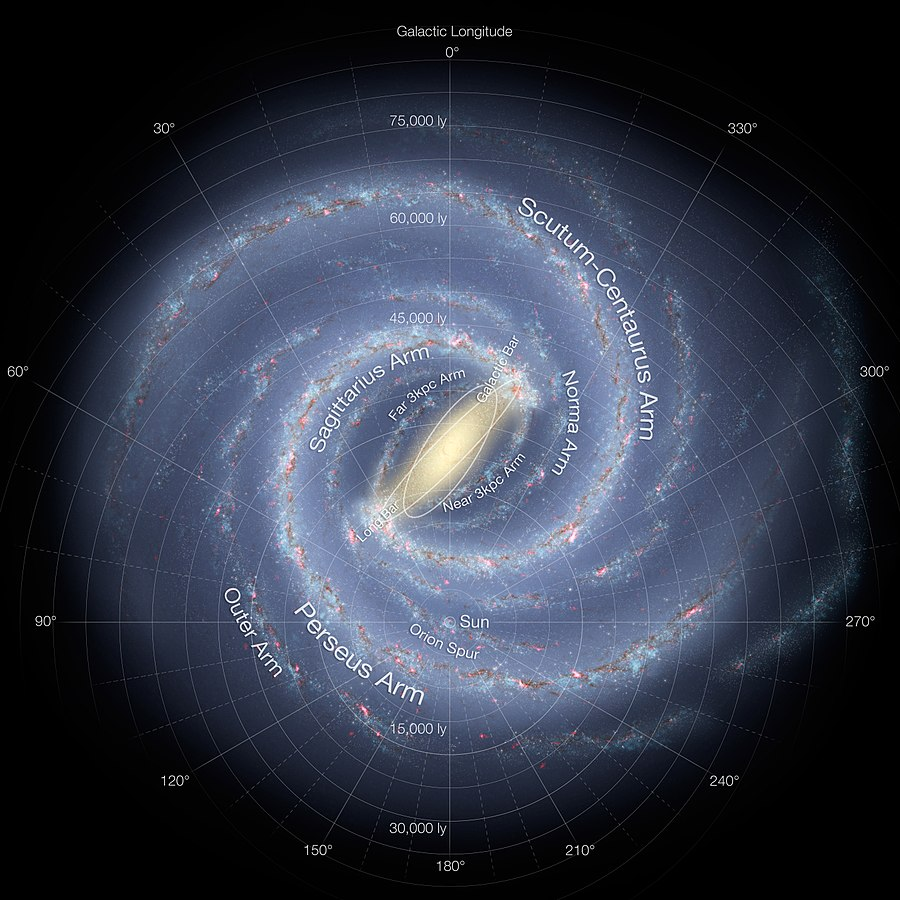
\includegraphics[width=0.5\linewidth]{milkyway.jpg}
\end{figure}
\end{frame}

%------------------------------------------------

\begin{frame}
\frametitle{Geometry of Galaxy}
\begin{figure}
\caption{Geometry of the Galaxy. C is Galactic center, S is Sun, M is gas cloud}
\includegraphics[width=0.5\linewidth]{galgeom}
\end{figure}
\end{frame}

%------------------------------------------------

\begin{frame}
\frametitle{Theory}
\begin{theorem}[Equation of Mapping the Milky Way]
$ \left\lbrace
\begin{array}{l}
	x=\mathit{r} \cos (\mathit{l}-90\degree) \\
	y=-\mathit{R}_{0}+\mathit{r} \sin (\mathit{l}-90\degree) \\
\end{array}
\right.$\\
This equation is for all galactic longitude $\mathit{l}$. Here $\mathit{R}_{0}$ is distance between Sun and galactic center and $\mathit{r}$ is distance to cloud from the Sun.
\end{theorem}
\end{frame}

%------------------------------------------------

\begin{frame}
\frametitle{Rotation Curve of a Galaxy}
\begin{figure}
\caption{Rotation curve of spiral galaxy Messier 33}
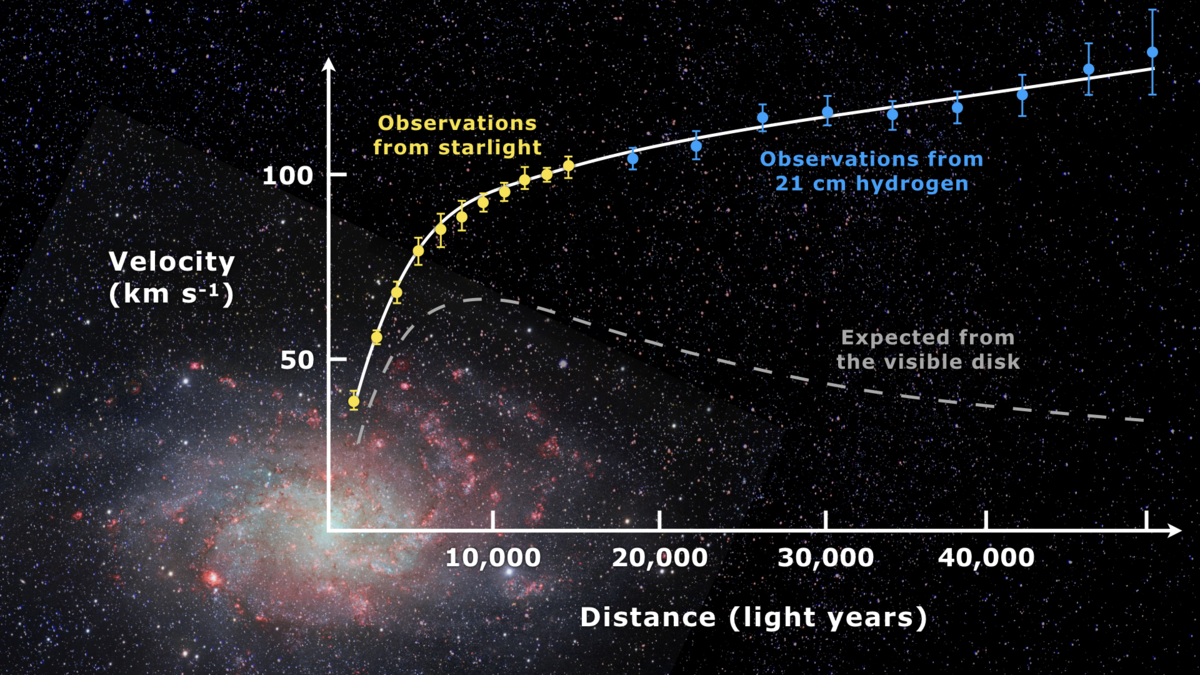
\includegraphics[width=0.8\linewidth]{rotcurve}
\end{figure}
\end{frame}

%------------------------------------------------

%------------------------------------------------

\section{Result of Experiment}

%------------------------------------------------

\begin{frame}
\frametitle{Galactic Mapping}
\begin{figure}
\caption{Mapping of Milky Way at $\mathit{l}=6\degree-225\degree$ and $\mathit{b}=0\degree$}
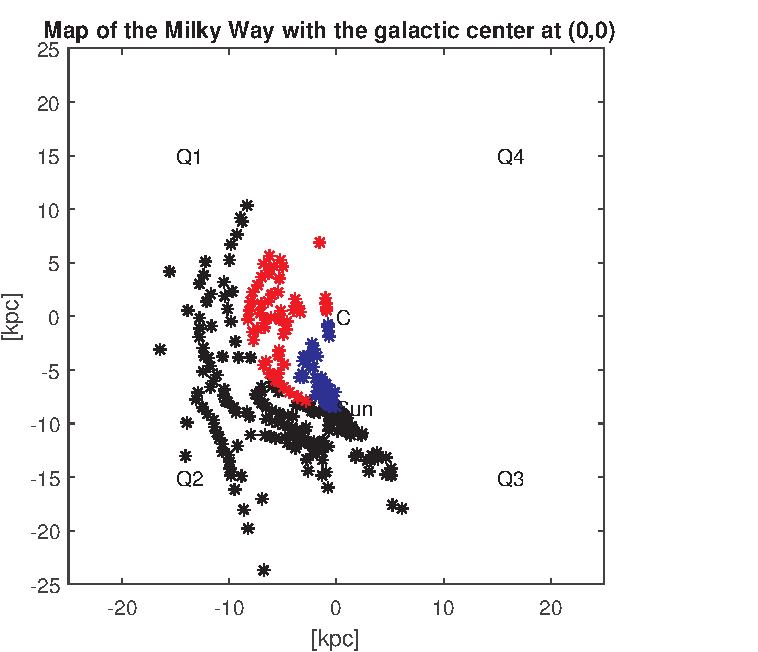
\includegraphics[width=0.6\linewidth]{map_1}
\end{figure}
\end{frame}

%------------------------------------------------

\begin{frame}
\frametitle{Galactic Rotation Curve}
\begin{figure}
\caption{Rotation Curve of Milky Way at $\mathit{l}=6\degree-225\degree$ and $\mathit{b}=0\degree$}
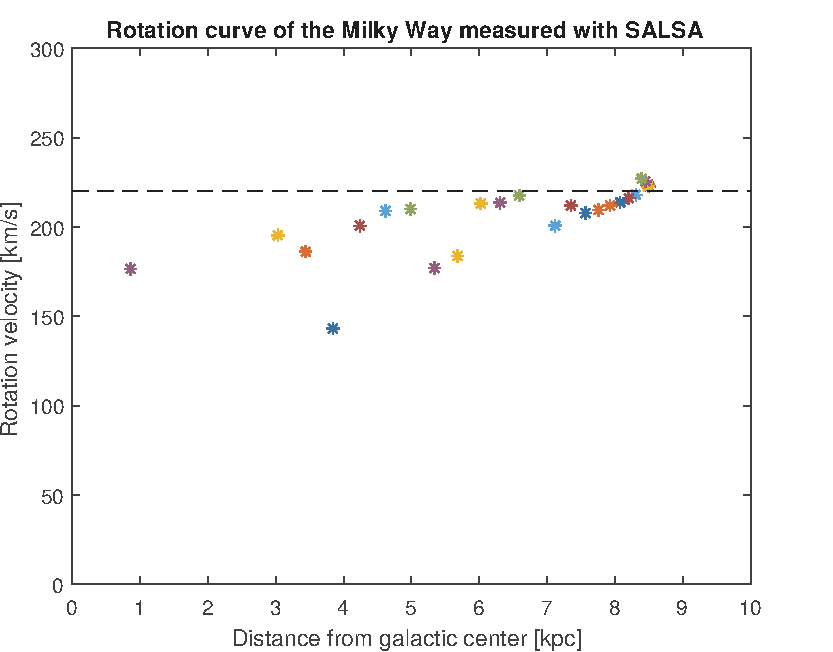
\includegraphics[width=0.6\linewidth]{rotationcurve_1}
\end{figure}
\end{frame}

%------------------------------------------------

%------------------------------------------------

\section{Importance of this Experiment}

%------------------------------------------------

\begin{frame}
\frametitle{Importance of this Experiment}
\begin{block}{Astrophysics Education}
Astrophysics students who are actually amateur level astronomers can evaluate galaxy dynamics and detect existence of dark matter in our galaxy easily with small radio telescope. This kind of practice can enlighten educators, students and enthusiasts.
\end{block}

\begin{block}{Amateur Astronomy and Citizen Science}
It will familiarize Observation of planetary radio signals, collecting solar flare data, meteor shower counts, GNSS satellite tracking, x-ray solar bursts detection etc to amateur astronomers and citizen scientists.
\end{block}

\begin{block}{STEM Education}
STEM students will learn about imaging techniques, signal processing, collecting data and analyze with computer programming and automation.
\end{block}
\end{frame}

%------------------------------------------------

%
%
%
%
%\begin{frame}
%\frametitle{Paragraphs of Text}
%Sed iaculis dapibus gravida. Morbi sed tortor erat, nec interdum arcu. Sed id lorem lectus. Quisque viverra augue id sem ornare non aliquam nibh tristique. Aenean in ligula nisl. Nulla sed tellus ipsum. Donec vestibulum ligula non lorem vulputate fermentum accumsan neque mollis.\\~\\
%
%Sed diam enim, sagittis nec condimentum sit amet, ullamcorper sit amet libero. Aliquam vel dui orci, a porta odio. Nullam id suscipit ipsum. Aenean lobortis commodo sem, ut commodo leo gravida vitae. Pellentesque vehicula ante iaculis arcu pretium rutrum eget sit amet purus. Integer ornare nulla quis neque ultrices lobortis. Vestibulum ultrices tincidunt libero, quis commodo erat ullamcorper id.
%\end{frame}
%%------------------------------------------------
%
%\begin{frame}
%\frametitle{Bullet Points}
%\begin{itemize}
%\item Lorem ipsum dolor sit amet, consectetur adipiscing elit
%\item Aliquam blandit faucibus nisi, sit amet dapibus enim tempus eu
%\item Nulla commodo, erat quis gravida posuere, elit lacus lobortis est, quis porttitor odio mauris at libero
%\item Nam cursus est eget velit posuere pellentesque
%\item Vestibulum faucibus velit a augue condimentum quis convallis nulla gravida
%\end{itemize}
%\end{frame}
%
%%------------------------------------------------
%
%
%
%%------------------------------------------------
%\section{Second Section}
%%------------------------------------------------
%
%\begin{frame}
%\frametitle{Table}
%\begin{table}
%\begin{tabular}{l l l}
%\toprule
%\textbf{Treatments} & \textbf{Response 1} & \textbf{Response 2}\\
%\midrule
%Treatment 1 & 0.0003262 & 0.562 \\
%Treatment 2 & 0.0015681 & 0.910 \\
%Treatment 3 & 0.0009271 & 0.296 \\
%\bottomrule
%\end{tabular}
%\caption{Table caption}
%\end{table}
%\end{frame}
%
%%------------------------------------------------
%
%\begin{frame}
%\frametitle{Theorem}
%\begin{theorem}[Mass--energy equivalence]
%$E = mc^2$
%\end{theorem}
%\end{frame}
%
%%------------------------------------------------

%%------------------------------------------------
%
%\subsection{Sample Code}
%
%%------------------------------------------------
%
%\begin{frame}[fragile] % Need to use the fragile option when verbatim is used in the slide
%\frametitle{Sample Code}
%\begin{example}[Theorem Slide Code]
%\begin{verbatim}
%\begin{frame}
%\frametitle{Theorem}
%\begin{theorem}[Mass--energy equivalence]
%$E = mc^2$
%\end{theorem}
%\end{frame}\end{verbatim}
%\end{example}
%\end{frame}
%
%%------------------------------------------------
%
%\begin{frame}
%\frametitle{Figure}
%Uncomment the code on this slide to include your own image from the same directory as the template .TeX file.
%%\begin{figure}
%%\includegraphics[width=0.8\linewidth]{test}
%%\end{figure}
%\end{frame}
%
%%------------------------------------------------
%
%\begin{frame}[fragile] % Need to use the fragile option when verbatim is used in the slide
%\frametitle{Citation}
%An example of the \verb|\cite| command to cite within the presentation:\\~
%
%%This statement requires citation \cite{p1}.
%\end{frame}
%
%
%%------------------------------------------------

%------------------------------------------------

\section{Conclusion}

%------------------------------------------------

\begin{frame}
\Huge{\centerline{Conclusion}}
\end{frame}

%----------------------------------------------------------------------------------------

%------------------------------------------------

\section{References}

%------------------------------------------------

\begin{frame}
\frametitle{References}
\footnotesize{
%\begin{thebibliography}{99} % Beamer does not support BibTeX so references must be inserted manually as below
%\bibitem[Smith, 2012]{p1} John Smith (2012)
%\newblock Title of the publication
%\newblock \emph{Journal Name} 12(3), 45 -- 678.
%\end{thebibliography}
%}
\bibliographystyle{IEEEtran}
\bibliography{mybibfile}}
\end{frame}

%------------------------------------------------

\begin{frame}
\Huge{\centerline{The End}}
\end{frame}

%----------------------------------------------------------------------------------------

\end{document}